\documentclass[11pt, a4paper]{article} 
\usepackage[utf8]{inputenc}
\usepackage[nolist,nohyperlinks]{acronym}
\usepackage{geometry}
\usepackage{setspace}

\usepackage{biblatex}
\usepackage[hidelinks]{hyperref}
\usepackage{nameref}

\usepackage{graphicx}
\usepackage{float}
\usepackage[hypcap=false]{caption}
\usepackage{subcaption}

\usepackage{tabularx}
\usepackage{multirow}

\usepackage{lipsum}

\usepackage{gensymb} % added by Steffen


\onehalfspacing
\addbibresource{arfeedback.bib}

% TabularX column defintions
\newcolumntype{L}[1]{>{\raggedright\let\newline\\\arraybackslash\hspace{0pt}}m{#1}}
\newcolumntype{C}[1]{>{\centering\let\newline\\\arraybackslash\hspace{0pt}}m{#1}}
\newcolumntype{R}[1]{>{\raggedleft\let\newline\\\arraybackslash\hspace{0pt}}m{#1}}

% Original assignment: Evaluate how to react on wrong AR usage
\newcommand{\mytitle}{Evaluation of Textual Feedback for Incorrect Usage of an Augmented Reality Application}
\newcommand{\runninghead}{Feedback for Augmented Reality}
\newcommand{\myauthor}{Julian Lüken, Mehmed Mustafa, Jan Schneider,\\ Steffen Tunkel, Chris Warin}
\newcommand{\myuni}{Georg-August University, Göttingen}
\newcommand{\titlespace}{1em}

% Header
\markright{\uppercase{\runninghead}\hfill}
\newenvironment{myabstract}{\begin{abstract}\begin{itshape}}{\end{itshape}\end{abstract}}

\begin{document}
	% Acronyms go here, refer to them with \ac{shorthand}
	\begin{acronym}
		\acro{AR}{Augmented Reality}
		\acro{SUS}{System Usability Scale}
	\end{acronym}

	\newgeometry{left=25mm,right=25mm,top=30mm,bottom=30mm}
	\pagestyle{empty}
	\begin{center}
		\begin{minipage}{.8\textwidth}
			\centering
			\begin{doublespace}\huge\textbf{\mytitle}\normalsize\\[\titlespace]\end{doublespace}
			\textsc{\myauthor}\\[\titlespace]
			\today\\[\titlespace]
			\myuni\\[\titlespace]
		\end{minipage}
	\end{center}
	\vspace{\titlespace}
	\begin{myabstract}
		% Abstract goes here
		\lipsum[1-3]
	\end{myabstract}
	\newgeometry{left=25mm,right=25mm,top=30mm,bottom=30mm}
	\pagestyle{myheadings}

	% REMEMBER
	%
	% Write in active, not passive
	% Write as "we"
	% Only two tenses (present and past)
	% Use LaTeX acronym environment (use \ac{shorthand} and define them right after \begin{document})
	% No paragraphs with only one sentence
	% No different types of paragraphs for pseudo-structuring
	% No forward references
	% Cite consistently and clearly (\cite{Lastname1999}, Jabref)
	% Footnotes: Just where really required
	% No repetitions

	\section*{Introduction}\label{sec:introduction}
		% Motivation
		% * Growing use of Augmented Reality and Lack of good feedback
		% * new technology: people don't yet know how to use AR features
		% * making AR usable without huge introductory efforts
		%
		% Research goals/questions
		% * To provide appropriate feedback to "wrong" AR usage/gestures
		% 	* To decide what type of feedback is better in comparison to other types
		%
		% Structure of report
		% * "For validation of our approach we conducted a usability case study"
		% * What will follow in the next sections
		%
		% moar sauce
		% https://www.statista.com/statistics/608967/mobile-ar-applications-installed-base-worldwide/
		% https://medium.com/iquii/augmented-reality-the-growth-through-smartphones-and-apps-and-the-future-for-businesses-ecb7dc9b17df
		%

		In recent years, the number of available mobile \ac{AR} applications for smartphones 
		has increased \cite{Tractica2017}. Although mobile \ac{AR} technology is no novelty, it was not widely available for 
		society until a variety of smartphones were capable of running AR applications. Since most 
		users are newly discovering \ac{AR} technology, they don't know how to use its features yet, thus using 
		unsupported gestures as input, which leads to frustration. Our main motivation for conducting this 
		research is the lack of good feedback in case of incorrect usage, which could help a lot of users to 
		avoid repeating common mistakes while using \ac{AR} applications for smartphones. Providing good feedback 
		could also help and teach users to control such \ac{AR} applications without the need of a separate introduction.

		Our research goal is to provide appropriate feedback to unsupported gestures and decide
		what type of textual feedback is the best. For validation of our approach we conducted a usability case study.

		The organization of the paper is as follows. The section \nameref{sec:foundations} gives information about
		usability in general and the \ac{AR} environment we provide the feedback for. In the section \nameref{sec:relatedwork} we discuss similar work on \ac{AR} and feedback done in the past. The \nameref{sec:approach} section
		gives a detailed illustration of the feedback we present to users. In the section \nameref{sec:casestudy}, we
		talk about the setup case study we conducted in order to validate our approach, followed by
		our results and the discussion thereof. Lastly, we summarize and conclude in the \nameref{sec:summary}.

	\section*{Foundations}\label{sec:foundations}
		% * What is AR?
		Since the main goal of our work presented in this paper is to find suitable user feedback for augmented reality environments, we will further clarify what \ac{AR} means and which technologies we used. \ac{AR} itself describes a variety of technologies that place 3D virtual objects into a 3D real environment in real time, for example via a handheld device like a mobile phone (mobile \ac{AR}) or using wearable goggles like the Microsoft HoloLens. In this paper we focus on \ac{AR} for mobile phones, where recorded imagery of the phone is being augmented and shown to the user to display a mix of virtual objects and the real world at runtime.


		% * Which frameworks/technologies were used?
		% 	* Brief info about Vivian (which relies on state machines)
		% 		* What gestures are "correct"? (vivian relies on 1 finger shit and moving environment)
		A virtual prototype is a \textit{"\textnormal{[…]} computer simulation of a physical product that can be presented, analyzed, and tested from concerned product life-cycle aspects such as design/engineering, manufacturing, service, and recycling as if on a real physical model."}\cite{Wang2002}. The Vivian framework is an extension for Unity3D, that can be used to create mobile \ac{AR} implementations of prototypes using a 3D model and one or more finite-state machines. (sauce?)

		\begin{figure}[H]
			\centering
			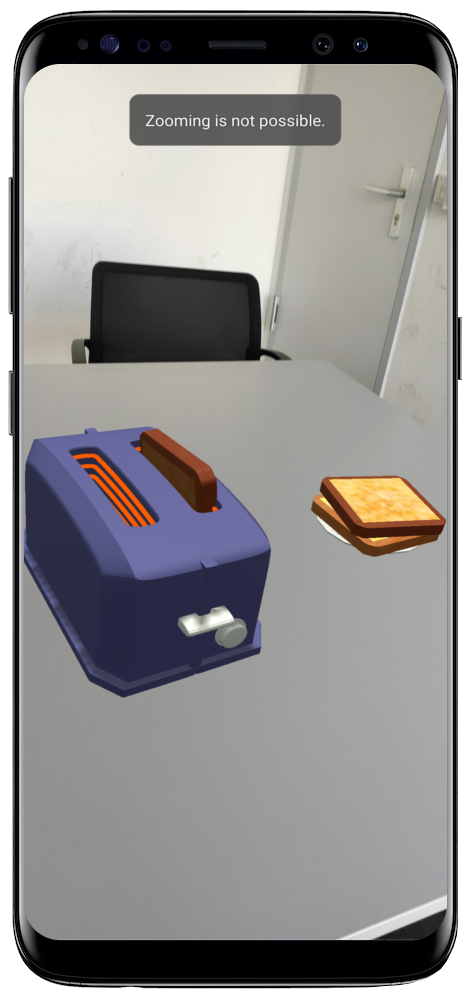
\includegraphics[width=.32\textwidth]{img/phone/phonepz1.png}
			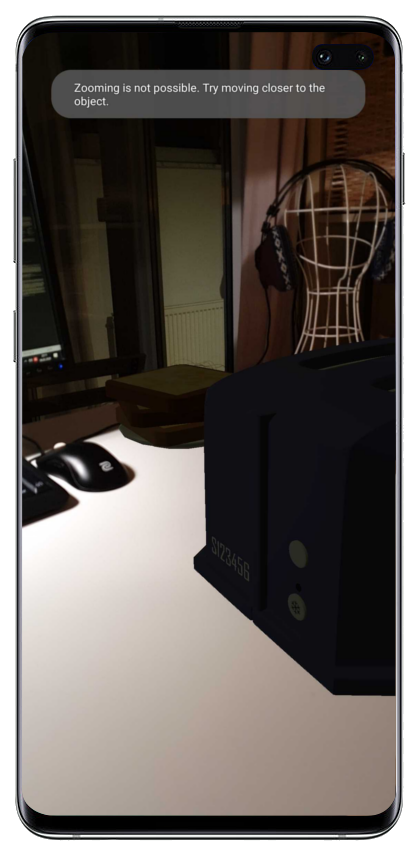
\includegraphics[width=.32\textwidth]{img/phone/phonepz2.png}
			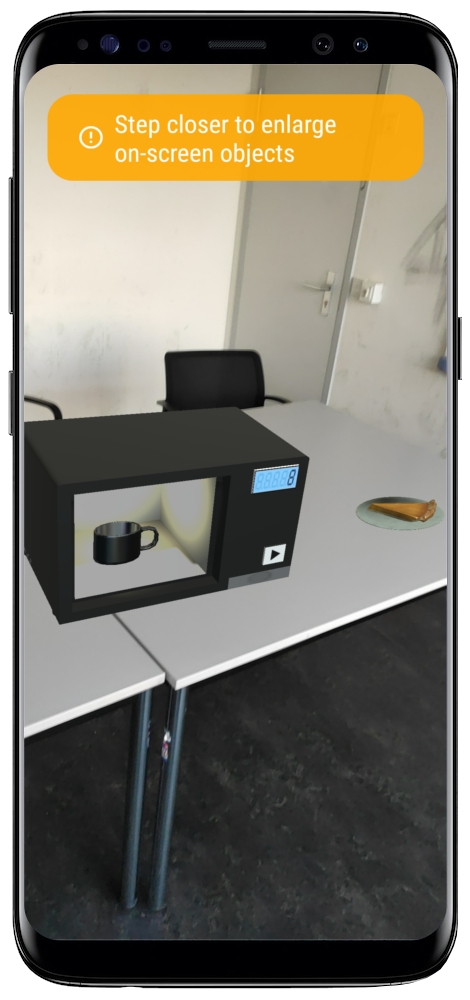
\includegraphics[width=.32\textwidth]{img/phone/phonepz3.png}
			\begin{subfigure}[t]{.32\textwidth}\centering
				\textbf{(A)}
			\end{subfigure}
			\begin{subfigure}[t]{.32\textwidth}\centering
				\textbf{(B)}
			\end{subfigure}
			\begin{subfigure}[t]{.32\textwidth}\centering
				\textbf{(C)}
			\end{subfigure}
			\caption{Three screenshots of an app made with the Vivian framework}
			\label{fig:feedbackonphone}
		\end{figure}

		In a mobile app made with the Vivian framework, all user input relies on one finger gestures on the touch screen. In the example in Figure \ref{fig:feedbackonphone} (A and B) we can observe a 3D model of a toaster projected onto a live video of a real world scenario using Vivian. The user can interact with the different 3D models on the screen. Buttons can be pressed by simply tapping the screen where the respective button is displayed. Knobs and levers can be moved by putting a finger on the screen where the knob or lever is displayed, moving the finger on the screen until finding the desired position, and removing the finger from the screen afterwards. We refer to this gesture as \emph{drag-and-drop}. The Vivian framework makes a clear distinction between movable and non-movable objects in a scene. The slice of bread in the aforementioned example is movable, whereas the toaster itself cannot be moved. Movable objects can be moved in the same fashion as a lever. To cover greater distances, one can move the device itself while dragging the object. Rotation similarly requires the user to hold their finger on the object and rotate the device until they find the desired orientation. The limit of one-finger-interactions exists due to the peculiarity of \ac{AR} environments where two-finger-interactions (like a pinch zoom or a two-finger-rotation) would be contradicting with the intended design of such an environment. If one wants to take a closer look at the previously mentioned toaster for example the user would need to step closer to the toaster.
		% * What is Usability(-testing)?
		% 	* Explain SUS (how did we tailor it to serve our purposes?)

		To evaluate different types of feedback, we decided to use usability testing as a tool to quantify the corresponding results. According to Nielsen, \textit{"usability is a quality attribute that assesses how easy user interfaces are to use. The word "usability" also refers to methods for improving ease-of-use during the design process."}\cite{Nielsen2012}. While usability testing refers to a \textit{"observational methodology to uncover problems and opportunities in designs"} with the goal to identify problems in the design of the product or service, uncover opportunities to improve and learn about the target user's behavior and preferences\cite{Moran2019}. Therefore we chose to have the users fill out a \ac{SUS} questionnaire which we tailored to fit our needs. The basic \ac{SUS} consists of ten questions regarding a systems usability. We added a few questions which target the feedback more as well as an open feedback item, where the participants were able to share their thoughts on the system with us. 
		% graphics:
		% * all feedback message types in response to one gesture (i.e. pinch zoom) for all prototypes, i.e.
		%	* toaster front view type 1 "pinch zoom"
		%	* toaster rear view type 2 "pinch zoom"
		%	* microwave front view type 3 "pinch zoom"
	\section*{Related Work}\label{sec:relatedwork}
		% Papers (as to be found in *.bib):
		% * Dey2016: A Systematic Review of 10 Years of Augmented Reality Usability Studies: 2005 to 2014 TODO remove
		% * Nilsson2007: Fun and Usable: Augmented Reality Instructions in a Hospital Setting
		% * Poupyrev2002: Developing a Generic Augmented Reality Interface
		The topic of error handling in \ac{AR}-applications has not been broadly studied yet. There are several guidelines on how to handle wrong user input. Microsoft states in its design guidelines, that error messages should alert users of an already occurred problem. Another point they make is that the message should be suppressed if it does not make the users change their behavior or perform an action\cite{Microsoft}. In addition to that, Nielsen's \textit{Error Message Guidelines} demand error messages to be phrased politely. This is to avoid the implication that the user did something stupid or inherently wrong. It is also important that the messages are precise descriptions of exact problems, offering constructive advice on how to fix the problem\cite{Nielsen2001}. A 2002 IEEE article discusses two approaches of how user help might be implemented in \ac{AR} environments. What they did was to offer an icon which the users might activate themselves when they seek advice for a given task. The other feature was an automated help message that pops up when the user moves an object associated to a certain task closer to his face and tilts it. They state, that \textit{"\textnormal{[t]}his approach is more suitable for AR interfaces than traditional desktop help systems, which either distract users with a constant barrage of help messages or interrupt their work by making them search explicitly for help."}\cite{IEEE2002}.

	\section*{Approach}\label{sec:approach}
		% What are "wrong" inputs? Which ones are "wrong"?
		% Describe feedback messages (size, color, content, duration) for each implementation <- graphics
		% Why these messages?
		% maybe a nice reference table for that too
		In order to find feedback in response to incorrect usage of a mobile \ac{AR} application, we have to define what kinds of gestures we consider incorrect in the first place. The user interface provided by the Vivian framework is based on one finger inputs (see \nameref{sec:foundations}), therefore we should take into consideration each input that is not done with a single finger. Prominent examples for multiple finger gestures are the \emph{pinch zoom} and the \emph{two finger rotation}. The pinch zoom is a gesture in which two fingers are placed on the touch screen and moved apart in opposite directions. The two finger rotation is a gesture in which two fingers are placed on the touch screen also and are together moved clockwise or counterclockwise about the center of the positions of the fingers. Common misconceptions by inexperienced mobile \ac{AR} users might include using said pinch zoom to either zoom in on objects or to bring them closer, or using two finger rotation to rotate objects.

		To make users quickly and easily understand the controls of Vivian-based apps, we extended the Vivian framework to provide three feedback message implementations that differ in content, colors and size. The content of the first feedback implementation is a \emph{critique}. If the user inputs a gesture that we consider incorrect, the app outputs a message that said input is not possible. For example, if a user tried pinch zooming, they would receive a message saying: "Pinch zooming is not possible". The content of the second feedback implementation is \emph{critique} and \emph{support}. We therefore refer to this feedback type as \emph{combined} in the course of this paper. The user is provided with a message stating that above mentioned input is not possible and hinting them towards what they should try instead. In the scope of the previous example, such a message would say: "Pinch zooming is not possible. Try moving around the object." In the first two implementations, the messages have the same size and color scheme (see Figure \ref{fig:feedbackonphone}, A and B). The third implementation is more concise \emph{support}. For our previous example the exact message is saying: "Step closer to enlarge on-screen objects." It also differs in color scheme and size (see Figure \ref{fig:feedbackonphone}, C). Each feedback message in every implementation is displayed for 5 seconds.

		\begin{center}
			\begin{tabular}{|C{.05\textwidth}|L{.15\textwidth}|L{.23\textwidth}|L{.45\textwidth}|} \hline
										& \textbf{Description}												& \textbf{Gesture (input)} 					& \textbf{Response (output)} 											\\ \hline
				\multirow{2}{*}{\#1}	& \multirow{2}{*}{\parbox{.15\textwidth}{critique}}					& two finger rotation						& Rotating the object is not possible.									\\ \cline{3-4}
										& 																	& pinch zoom								& Zooming is not possible. 												\\ \hline
				\multirow{2}{*}{\#2}	& \multirow{2}{*}{\parbox{.15\textwidth}{combined}}					& two finger rotation						& Rotating the object is not possible. Try moving around the object.	\\ \cline{3-4}
										& 																	& pinch zoom								& Zooming is not possible. Try moving closer to the object.				\\ \hline
				\multirow{3}{*}{\#3}	& \multirow{3}{*}{\parbox{.15\textwidth}{support}}					& two finger rotation (movable object)		& Hold the phone and move the object to rotate							\\ \cline{3-4}
										& 																	& two finger rotation (elsewhere)			& Move around the objects												\\ \cline{3-4}
										&																	& pinch zoom 								& Step closer to enlarge on-screen objects								\\ \hline
			\end{tabular}
			\captionof{table}{The responses for each input in each implementation.}
			\label{tab:feedback}
		\end{center}

		The contents of each message can be found in Table \ref{tab:feedback}. The description column holds the names we assigned to the three different feedback implementations. In the gesture and response columns you can find the corresponding inputs and outputs respectively. If for example a user tried a two finger rotation in the critique implementation, the app would display a message saying "Rotating the object is not possible".
		In the support implementation we made the distinction between two finger rotations on movable objects and elsewhere. If the aforementioned center point of the two finger rotation is placed on a movable object (see \nameref{sec:foundations}), the app displays the message that corresponds to "two finger rotation (movable object)". If the two finger rotation is executed elsewhere, the "two finger rotation (elsewhere)" message is displayed instead.

	\section*{Case Study}\label{sec:casestudy}
		% --> Steffen has to add some real text right here.
		%
		% SETUP
		% * introduce prototypes
		%	* functionalities
		%
		% * introduce groups(+subgroups)
		%	* size
		%	* what do they do
		%	* naming conventions
		%
		% * introduction to participants
		%
		% * tasks (hints)
		%
		% * what do we measure and how? 
		%	* screen recordings
		%	* notepad
		%
		% * questionnaire
		%	* SUS
		%	* open question
		%
		%
		% RESULTS
		% * first proto toaster
		% * first proto microwave
		% * second proto toaster
		% * second proto microwave
		%
		% * did wrong once vs did wrong multiple times
		%
		% * time to fulfill task per level
		% * time to fulfill tasks per prototype order
		% * number of wrong usages per level
		% * percentage of which group asking for more feedback
		% 
		% DISCUSSION
		% * hypothesis "visible and better feedback msg help the user to fulfill tasks faster, easier"
		% * feedback message must be genera enough to be applicable to any possible situation
		% * feedback message must be specific enough to be more helpful in the given situation
		% * outlines: sus/free answers
		% * easy prototype microwave -> intuitively usable, no feedback needed
		%
		% THREATS TO VALIDTY
		%
		\subsection*{Setup of the Case Study}\label{ssec:setup}
			To evaluate the quality of our feedback implementations we conducted a case study in the domain of usability engineering. We used two different prototypes supported by the Vivian Framework (see \nameref{sec:foundations}). Both of them are quite simple kitchen devices: a toaster prototype and a microwave prototype (as seen in Figure \ref{fig:feedbackonphone}).

			The microwave's functionality is limited to heating an object inside it with constant power. It has one button to add 10 seconds to the heating duration and one to open the door. The door can be closed by moving it. The status of the microwave is visually indicated by a small display showing the remaining heating time and a light inside the device, which turns on when it is open or heating. The toaster can toast one or two pieces of bread at a time. The toasting can be started by pulling down a handle and stopped by pushing it up again or by pressing the stop button, which is on the backside. Otherwise, the toasting stops automatically after a time which is defined by the position of a rotatable knob. The time mode is divided into 'low', 'medium' and 'high'. Further functionality is provided by the unfreezing mode, which can be activated by the snowflake button on the backside. The activation of the unfreezing mode results in a longer toasting duration and is indicated by a light above the button. The toasting process itself is displayed by the glowing of the heating elements. Both prototypes have a serial number on the backside. Both scenes contain different additional objects, which the user can interact with. These are pieces of bread for the toaster and for the microwave a cup which is already inside the microwave in the beginning and a piece of cake next to it.
			
			\begin{center}
				\begin{tabular}{|C{.05\textwidth}|L{.41\textwidth}|L{.41\textwidth}|}
					\hline \textbf{\#} & \textbf{Microwave} & \textbf{Toaster} \\
					\hline 1 & Read serial number off the microwave & Read serial number off the toaster \\
					\hline 2 & Heat up the cup & Toast the bread \\
					\hline 3 & Remove the cup, put the pie in, set the timer to 20 seconds and remove the plate at 5 seconds & Toast the bread on high heat and put the toaster in unfreezing mode \\
					\hline
				\end{tabular}
				\captionof{table}{The tasks for the different prototypes.}
				\label{tab:tasks}
			\end{center}

			Based on these functionalities we designed 3 tasks per prototype, which are shown in Table \ref{tab:tasks}. Important about this tasks is that they are increasing in complexity. An example of this increase is that task 2 of the microwave asks to heat the cup, which is already in the microwave, for any time. Therefore just the start button has to be pressed once to fulfill the task. Afterwards, task 3 is to replace the cup by the pie and heat for a specific time. This contains a lot more necessary steps: open the door, move the cup out, move the pie in, close the door, press the start button multiple times and finally also press the stop button after the desired time is over.

			For the case study, we divided the participants into 4 groups. Each of these groups tested another version of the feedback implementation. We gave no feedback at all to the participants in group 0. Participants in group 1 got our first implementation with \emph{critique} like feedback, in group 2 they got our second implementation with a \emph{combined} feedback version and in group 3 they got our third implementation with a \emph{supportive} feedback (see \nameref{sec:approach}). Each participant was asked to fulfill the tasks for each prototype in the order provided in Table \ref{tab:tasks}. One half of the participants were asked to do the tasks of the toaster prototype first, while the other half did the tasks for the microwave prototype first. We were able to evaluate subgroups with a certain implementation level and a certain order of prototypes they tested. In the following, the subgroups are named \emph{TM}, which translates to "first toaster, then microwave" and \emph{MT}, which translates to "first microwave then toaster", followed by the number of their feedback group. For example, a participant who was assigned the toaster first and then the microwave without any feedback was in the subgroup TM0.

			Before the actual start of the test, we gave every participant a short introduction. This introduction contains information about the \ac{AR} technology and reasons behind usability testing to prepare the participants and create a similar level of expectation. It deliberately does not contain any information about how to use the application or the scope of the case study. This is important so the participants are not biased about wrong usage and the feedback they would get. During the test, we used screen recordings to measure each participants use of the application. These enabled us to acquire completion times for the different tasks and count the number of wrong usages. We used a notepad to register further observations.

			Following the test of the application the participants were asked to fill in a questionnaire. This questionnaire consists of 3 parts. First we asked participants if they have used \ac{AR} applications before. The second part is an \ac{SUS} (see \nameref{sec:foundations}) about the usability of the \ac{AR} application. The third part is an open question directly aimed to the feedback provided by the application, namely: \emph{"If you have any suggestions on what kind of feedback from the app you would find better, please let us know"}.

			We conducted the case study with 10 participants per group of feedback implementation. This leads to 40 people participating in the case study in total. The smallest sub groups, defined by implementation and task order, were still filled with 5 participants.

		\subsection*{Results of the Case Study}\label{ssec:results}
			% only pure results and graphics
			% shall provide base for discussion
			In our approach we consider especially two gestures as incorrect usage, the pinch zoom and the two finger rotation (see \nameref{sec:approach}). With the setup of our case study the two finger rotation appeared more often than the pinch zoom gesture. In total over all participants and all tasks, two finger rotations appeared 225 times, while pinch zoom just appeared 51 times. Since 82\% of the incorrect usages are two finger rotations, the results of our case study concentrate on those. We especially evaluate the 2nd task for the toaster since it was most demanding for the users. As shown in diagram \ref{fig:tfr_v_pz}, 91\% of the overall two finger rotations occurred in that task. Also the majority of pinch zoom gestures occurred there.

			\begin{figure}[H]
						\centering
						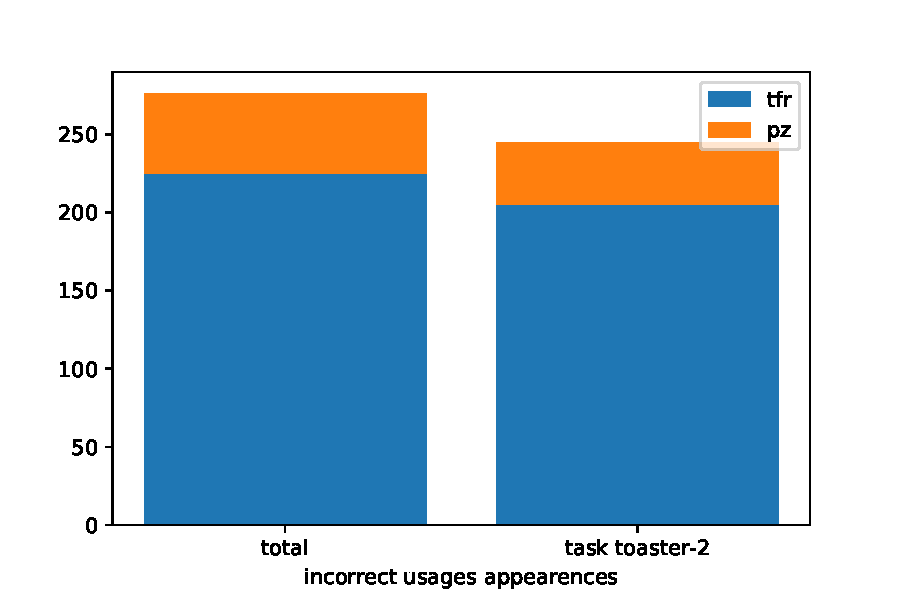
\includegraphics[width=.49\textwidth]{img/plot/plot_tfr_v_pz.pdf}
						\caption{DUMMY: Appearances of two finger rotations and pinch zooms in total and for the 2nd task for the toaster prototype.}
						\label{fig:tfr_v_pz}
					\end{figure}


			To evaluate the effectiveness of the different implementations we compare the users behavior for the 2nd task of the toaster, with different measures. Diagram \ref{fig:t2_metrics} shows the two most important measures. Diagram \ref{fig:t2_metrics}-A gives the mean time needed for the task with the different implementations. The black lines on the bar plot give additional information with the standard deviation for each implementations time. Diagram \ref{fig:t2_metrics}-B is similar. This diagram shows the mean values of two finger rotation tries per user for the different implementations. Also here the black lines on the bars give the standard deviation for each of this values. Important for this graph is that users, who had zero two finger rotation attempts, are excluded from the statistic. The reason behind it is, that these users didn't receive any feedback message independent of their given implementation. To trigger any feedback a incorrect usage must appear at least once. In total 4 of the 40 participants didn't tried any two finger rotations on this task. The maximal number for one specific implementation is 2. That means for each implementation at least 8 participants data was used to take the statistical values.

			\begin{figure}[H]
						\centering
						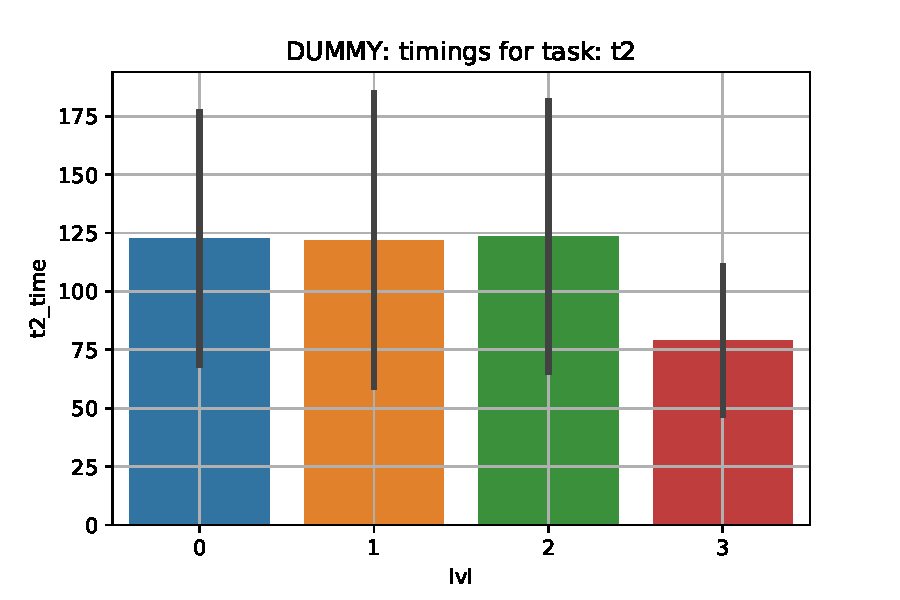
\includegraphics[width=.49\textwidth]{img/plot/plot_time_barplot.pdf}
						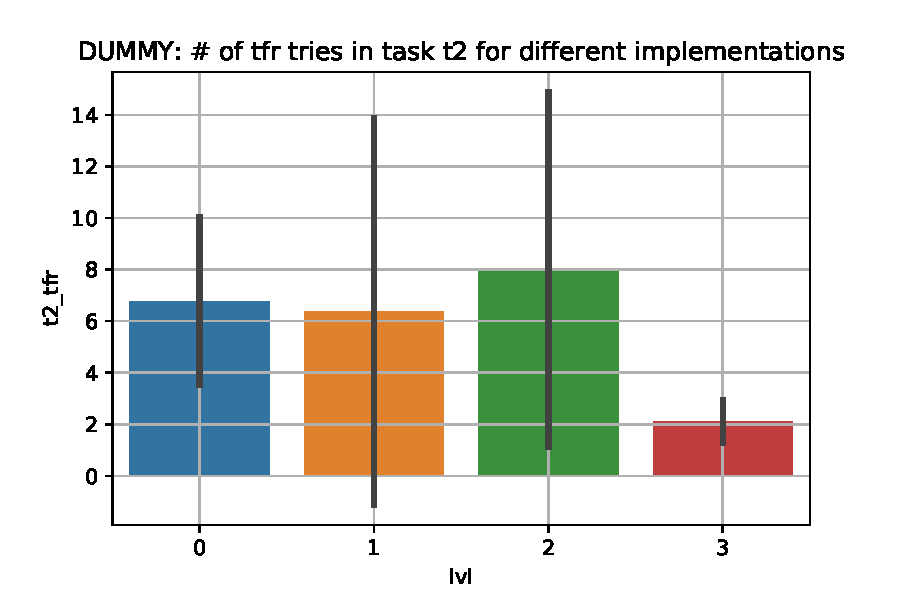
\includegraphics[width=.49\textwidth]{img/plot/plot_tfr_barplot.pdf}
						\begin{subfigure}[t]{.49\textwidth}\centering
							\textbf{(A)}
						\end{subfigure}
						\begin{subfigure}[t]{.49\textwidth}\centering
							\textbf{(B)}
						\end{subfigure}
						\caption{DUMMY: Evaluation of the time and two finger rotation tries needed for the 2nd task for the toaster prototype}
						\label{fig:t2_metrics}
					\end{figure}

			To check, whether the result is statistically significant we perform statistical tests on both, the time needed for the task and the number of two finger rotation attempts. The main test is \emph{Welch t-test} to compare the different implementations with the zero group, which didn't receive any kind of feedback messages. \emph{Welch t-test} has the assumption that both populations are normally distributed. We used the \emph{Shapiro-Wilk} test on the residuals between the given implementations group and the zero feedback group. Generally we consider p-values below 0.05\% as statistically significant. Table \ref{fig:stats} shows the p-values of the tests for the implementation with \emph{concise} feedback (used by group 3). We focus on this results because the mean values of this implementations metrics implicate the biggest difference to the zero feedback group. Since all of the p-values of the \emph{Shapiro-Wilk} test are above the threshold, the normality assumption for \emph{Welch t-test} holds. The result of the \emph{Welch t-test} for the number of two finger rotation tries in task 2 of the toaster implies a significant difference to the zero group, which can not be confirmed by the result for the timings for the task.

			\begin{figure}[H]
						\centering
						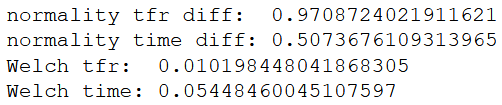
\includegraphics[width=.49\textwidth]{img/stats_table_dummy.png}
						\caption{DUMMY: p-values for Shapiro-Wilk test and Welch t-test with both metrics}
						\label{fig:stats}
					\end{figure}

			In addition we evaluate the relationship between our two metrics for the task. The correlation coefficient between the both is 0.43, which indicates a moderate positive relationship between the metrics. Diagram \ref{fig:scatter} visualizes the relationship between the time needed for the task and the number of two finger rotation tries. The color of a data point is set by the implementation used by this participant. It is visible that the participants with implementation 3 are all clustered with a low time and a low amount of two finger rotations, while all other groups are more randomly spread.

			\begin{figure}[H]
						\centering
						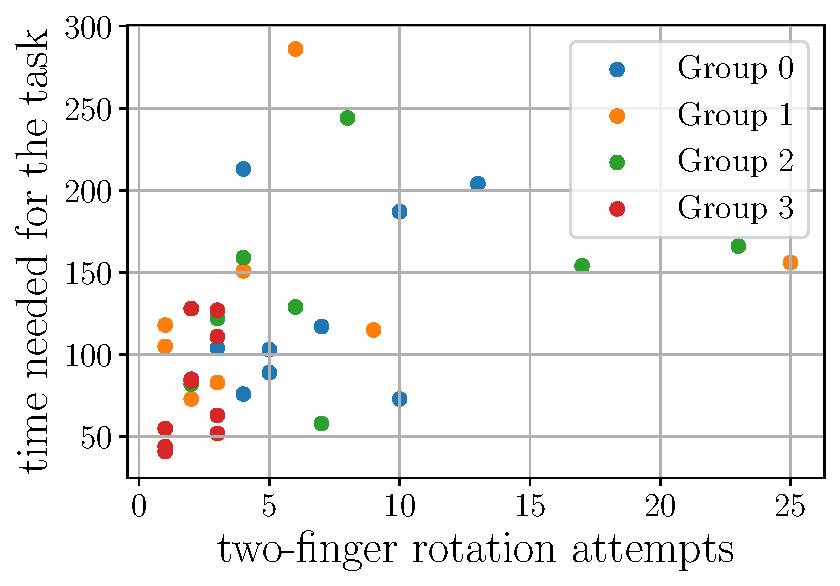
\includegraphics[width=.49\textwidth]{img/plot/plot_scatter.pdf}
						\caption{DUMMY: Time needed to fulfill the 2nd task for the toaster prototype depended on the number of tfr tries.}
						\label{fig:scatter}
					\end{figure}

			For the evaluation of the questionnaire we calculate the \ac{SUS} scores for every participant. Diagram \ref{fig:sus} shows the scores mean for each implementation. The horizontal red line is at a score of 68, which means average usability.

			\begin{figure}[H]
						\centering
						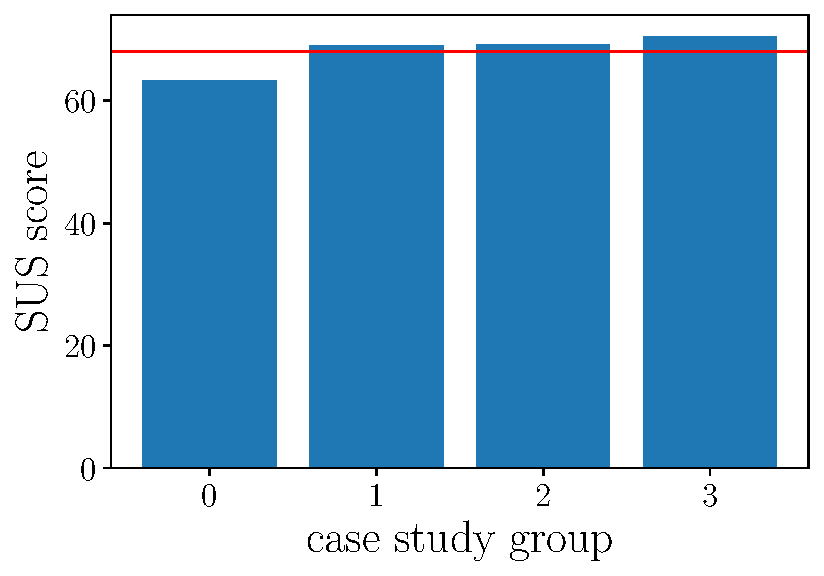
\includegraphics[width=.49\textwidth]{img/plot/plot_sus.pdf}
						\caption{DUMMY: SUS score for different implementations.}
						\label{fig:sus}
					\end{figure}

			24 of the 40 participants answered the open question (\emph{"If you have any suggestions on what kind of feedback from the app you would find better, please let us know"}). We categorize the answers with 4 different labels, divided by the topic the answer is about. These are \emph{app feedback}, \emph{app controls}, \emph{prototype design} and \emph{other}. The appearances of the different types of answers are listed in diagram \ref{fig:tags}. In case an answer fit to multiple labels, we counted it for all the fitting categories. In addition to the type of answer we also take the implementation the participant tested and the specific text into account to gain knowledge from them. 

			\begin{figure}[H]
						\centering
						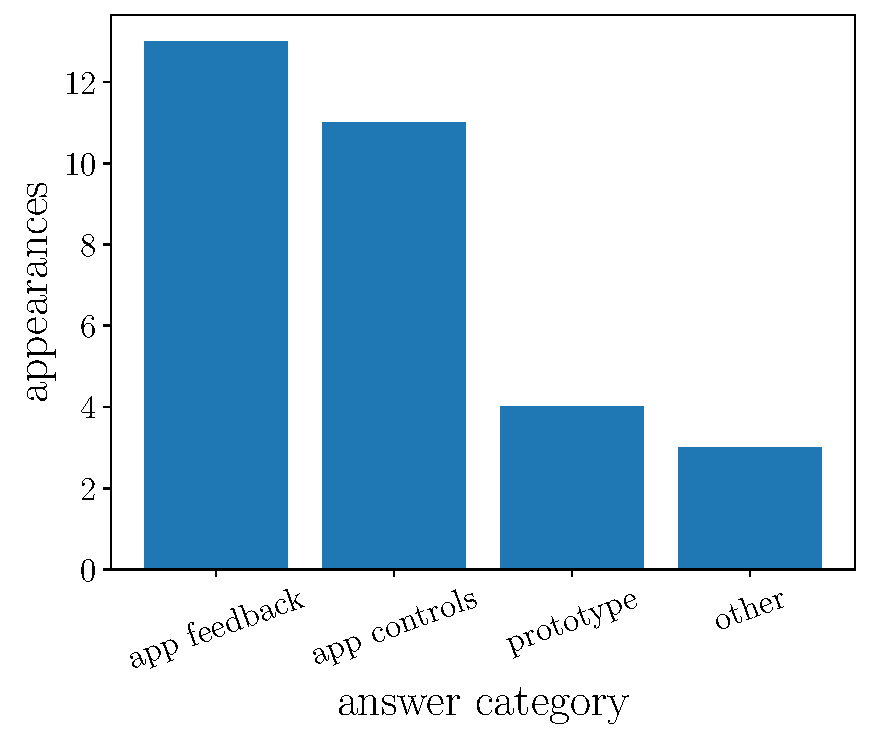
\includegraphics[width=.49\textwidth]{img/plot/plot_tags.pdf}
						\caption{DUMMY: Amount of open question answers categorized by labels.}
						\label{fig:tags}
					\end{figure}

		\subsection*{Discussion of the Case Study Results}\label{ssec:discussion}
			% discussion of the results in the previous section
			% "threads to validity" part
			\iffalse
			With the given setup of our case study its not surprising, that the two finger rotation gesture appeared more often than the pinch zoom. Usually users attempt the pinch zoom gesture when an object on the screen is to small to see or use. Our participants started right in front of the object, so there was no need to step a lot closer to it. Also the prototype are not created with unnecessary small controls, which means all of them are good visible in general. Clearly there are other applications where users are more tempted to use this gesture. It is likely that outcomes of the evaluation of feedback messages for incorrect usages for rotation are applicable in a similar way for zoom and other functionalities. For the evaluation of the rotation we have to divide it into two groups, as we do for our \emph{concise} feedback implementation (see \nameref{sec:approach}). While most of the users intuitively walked around objects to rotate their view on the scene, they struggled more with rotating a certain object. This is the reason why the 2nd task for the toaster prototype is most important in the task setup. The specific task is just "Toast a toast", but this includes rotating the laying object by $90\degree$ to put it into the device. The struggle with this task also becomes visible by the fact that only 10\% of the participants were able to do it intuitively without trying a two finger rotation before.
			[a lot is missing here]
			\fi

	\section*{Summary and Outlook}\label{sec:summary}
		\cite{Dey2016} \cite{Nilsson2007} \cite{Poupyrev2002} \ac{AR} \ac{AR}

	\pagebreak
	\printbibliography
\restoregeometry
\end{document}